In this chapter we will outline the project management plan from initiation to delivery.

\section{Project Management Plan Outline}
\label{ch:projectplanoutline}

The project management plan is split into five distinct phases shown in figure \ref{fig:projectphases}. The first stage is the initiation phase outlined in \ref{ch:projectinitiation}. It contains the groundwork so the project can go ahead. No specific planning of project work is done in this phase. The second phase contains the planning of the project work and is detailed in \ref{ch:planningphase}. This includes scope management, quality management, project schedule and communications management. In the execution phase described in \ref{ch:executionphase} the project work gets carried out. It entails progress and communications management. The fourth phase is called "Monitoring and Controlling" and describes all actions that need to take place alongside all other phases. This includes, among other things, the validation and control of the scope, quality and schedule defined in the planning phase. The last phase detailed in \ref{ch:projectclosing} entails all steps that need to take place in order to deliver the final product, such as demonstration and final presentation.

\begin{figure}
  \centering
  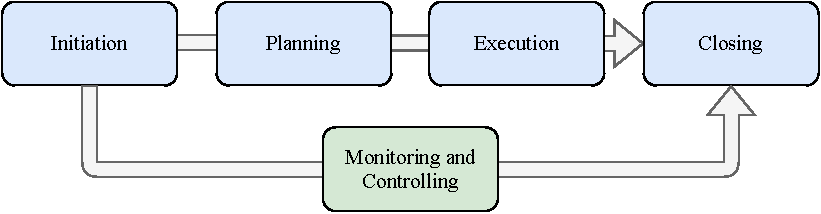
\includegraphics{data/figures/project_lifecycle.pdf}
  \caption{Project Phases}
  \label{fig:projectphases}
\end{figure}


\section{Project Initiation}
\label{ch:projectinitiation}

\section{Planning Phase}
\label{ch:planningphase}

\section{Execution Phase}
\label{ch:executionphase}

\section{Monitoring and Controlling}
\label{ch:monitoringcontrolling}

\section{Project Closing and Delivery}
\label{ch:projectclosing}
